\documentclass[english]{article}
\usepackage[T1]{fontenc}
\usepackage[latin9]{inputenc}
\usepackage{amstext}
\usepackage{babel,color}
\usepackage{amsmath}
\usepackage{amssymb}
\usepackage{geometry}
\usepackage{graphicx}
\usepackage{epstopdf}
\geometry{letterpaper,tmargin=1in,bmargin=1in,lmargin=1in,rmargin=1in}
%\usepackage[parfill]{parskip}    % Activate to begin paragraphs with an empty line rather than an indent
\parskip = 0.03in

\newtheorem{theorem}{Theorem}

\input my_header.tex

\begin{document}

\section*{Unprocessed Rank-1 Matched Oracle Classifier}

We consider the following binary classification problem:

\begin{equation}
y=\left\{
\begin{aligned}
&z
&& y\in H_0\\
&u_1x+z
&& y\in H_1\\
\end{aligned}\right.
\end{equation}

where $u_1\in\mathbb{C}^n$, $\|u_1\|^2=1$, $z\sim\mathcal{N}(0,I)$, $x\sim\mathcal{N}(0,\sigma^2)$. We assume that $x$ and $z$ are independent and that$u_1$ is known.

Under $H_0$, $y\sim\mathcal{N}(0,I)$ and under $H_1$ $y\sim\mathcal{N}(0,\sigma^2u_1u_1^H+I)$.

Our LRT is

\begin{equation}
\begin{aligned}
&\Lambda(y)
&&=\frac{\left(2\pi\right)^{-n/2}|\sigma^2u_1u_1^H|^{-1/2}\exp\{-\frac{1}{2}y^H\left(\sigma^2u_1u_1^H+I\right)^{-1}y\}}{\left(2\pi\right)^{-n/2}\exp\{-\frac{1}{2}y^Hy\}}\\
&&&=|\sigma^2u_1u_1^H|^{-1/2}\exp\{-\frac{1}{2}y^H\left[\left(\sigma^2u_1u_1^H+I\right)^{-1}-I\right]y\}
\end{aligned}
\end{equation}

where our decision is

\begin{equation}
\begin{aligned}
&\text{Declare } H_0 \text{ if}
&& \Lambda(y) < \eta\\
& \text{Declare } H_1 \text{ if}
&& \Lambda(y) > \eta\\
\end{aligned}
\end{equation}

Taking the log of both sides and rearranging yields

\begin{equation}
\begin{aligned}
&\ln\left(\Lambda(y)\right)=\tilde{\Gamma(y)}
&&=y^H\left[I-\left(\sigma^2u_1u_1^H+I\right)^{-1}\right]y
\end{aligned}
\end{equation}

Defining $\gamma = 2\ln(\eta)+\ln(|\sigma^2u_1u_1^H|)$ we have the decision

\begin{equation}
\begin{aligned}
&\text{Declare } H_0 \text{ if}
&& \tilde{\Lambda}(y) < \gamma\\
& \text{Declare } H_1 \text{ if}
&& \tilde{\Lambda}(y) > \gamma\
\end{aligned}
\end{equation}

Using the Woodberry matrix inversion formula, we have

\begin{equation}
\left(\sigma^2u_1u_1^H+I\right)^{-1}= I - \sigma^2u_1(1+\sigma^2u_1^HIu_1)^{-1}u_1^H=I-\frac{\sigma^2u_1u_1^H}{1+\sigma^2u_1^Hu_1}
\end{equation}

Our statistic becomes

\begin{equation}\label{eq:unproc oracle}
\boxed{\tilde{\Lambda}(y)=\frac{\sigma^2y^Hu_1u_1^Hy}{1+\sigma^2}}
\end{equation}

\section*{Unprocessed Rank-1 Matched Plug-in Classifier}

As often is the case, we do not know $u_1$ explicitly and must make an estimate $\hat{u}_1$ from training data. One simply solution when doing so, is to simply plug in the estimate wherever necessary in our optimal detector. This yields the following plug-in detector

\begin{equation}\label{eq:unproc plugin}
\boxed{\hat{\Lambda}(y)=\frac{\sigma^2y^H\hat{u}_1\hat{u}_1^Hy}{1+\sigma^2}}
\end{equation}

with the decision

\begin{equation}
\begin{aligned}
&\text{Declare } H_0 \text{ if}
&& \hat{\Lambda}(y) < \gamma\\
& \text{Declare } H_1 \text{ if}
&& \hat{\Lambda}(y) > \gamma\
\end{aligned}
\end{equation}

\section*{Processed Rank-1 Matched Oracle Classifier}

Again, we consider the problem

\begin{equation}
y=\left\{
\begin{aligned}
&z
&& y\in H_0\\
&u_1x+z
&& y\in H_1\\
\end{aligned}\right.
\end{equation}

and consider the processed data, $w=\hat{u}_1^Hy$. Under $H_0$, $w\sim\mathcal{N}(0,1)$ and under $H_1$, $w\sim\mathcal{N}(0, \sigma^2|<\hat{u}_1,u_1>|^2+1)$

Our LRT is

\begin{equation}
\begin{aligned}
&\Lambda(w)
&&=\frac{\left(2\pi(\sigma^2|<\hat{u}_1,u_1>|^2+1)\right)^{-1/2}|\sigma^2u_1u_1^H|^{-1/2}\exp\{-\frac{1}{2(\sigma^2|<\hat{u}_1,u_1>|^2+1)}w^2\}}{\left(2\pi\right)^{-1/2}\exp\{-\frac{1}{2}w^2\}}\\
&&&=(\sigma^2|<\hat{u}_1,u_1>|^2+1)^{-1/2}\exp\{-\frac{1}{2}w^2\left[\left(\frac{1}{\sigma^2|<\hat{u}_1,u_1>|^2+1}-1\right)\right]\}
\end{aligned}
\end{equation}

with the decision

\begin{equation}
\begin{aligned}
&\text{Declare } H_0 \text{ if}
&& \Lambda(y) < \eta\\
& \text{Declare } H_1 \text{ if}
&& \Lambda(y) > \eta\\
\end{aligned}
\end{equation}

Taking the log of both sides and rearranging yields

\begin{equation}
\tilde{\Lambda}(w) = w^2\left(\frac{\sigma^2|<\hat{u}_1,u_1>|^2}{\sigma^2|<\hat{u}_1,u_1>|^2+1}\right)
\end{equation}

Observing that $\frac{\sigma^2|<\hat{u}_1,u_1>|^2}{\sigma^2|<\hat{u}_1,u_1>|^2+1}$ is simply constant, our statistic is

\begin{equation}\label{eq:proc oracle}
\boxed{\tilde{\Lambda}(w) = w^2}
\end{equation}

and defining $\gamma = 2\left(\frac{\sigma^2|<\hat{u}_1,u_1>|^2+1}{\sigma^2|<\hat{u}_1,u_1>|^2}\right)\ln\left(\eta\left(\sigma^2|<\hat{u}_1,u_1>|^2+1\right)^{1/2}\right)$ our decision becomes

\begin{equation}
\begin{aligned}
&\text{Declare } H_0 \text{ if}
&& \tilde{\Lambda}(y) < \gamma\\
& \text{Declare } H_1 \text{ if}
&& \tilde{\Lambda}(y) > \gamma\\
\end{aligned}
\end{equation}

\section*{Processed Rank-1 Matched Plug-in Classifier}

Our plug-in classifier assumes that $\hat{u}_1=u_1$ and thus that $|<\hat{u}_1,u_1>|^2=1$. Plugging this into our oracle classifier yields
\begin{equation}\label{eq:proc plugin}
\boxed{\hat{\Lambda}(w) = w^2}
\end{equation}

with the decision

\begin{equation}
\begin{aligned}
&\text{Declare } H_0 \text{ if}
&& \hat{\Lambda}(y) < \gamma\\
& \text{Declare } H_1 \text{ if}
&& \hat{\Lambda}(y) > \gamma\\
\end{aligned}
\end{equation}

where $\gamma = 2\left(\frac{\sigma^2+1}{\sigma^2}\right)\ln\left(\eta\left(\sigma^2+1\right)^{1/2}\right)$ is our threshold. Recalling that $w=\hat{u}_1^Hy$, we observe that this is the same as the plug-in classifier in (\ref{eq:unproc plugin}).

\section*{Theoretical ROC for (\ref{eq:proc plugin}) and (\ref{eq:proc oracle})}

In both (\ref{eq:proc plugin}) and (\ref{eq:proc oracle}) our statistic, $\hat{\Lambda}(w)$, is $w^2$. Clearly in this rank-1 setting, our plug-in detector is optimal. We derive the theoretical ROC for this detector. Under $H_0$ we have that $w\sim\mathcal{N}(0,1)$. Therefore $w^2\sim\chi^2_1$.

Our probability of false alarm is

\begin{equation}
\begin{aligned}
&P_F
&&=P(\tilde{\Lambda}(w) >\gamma|H_0) \\
&&&= P\left(w^2\left(\frac{\sigma^2|<\hat{u}_1,u_1>|^2}{\sigma^2|<\hat{u}_1,u_1>|^2+1}\right)>\gamma|H_0\right)\\
&&&=P\left(w^2>\gamma\left(\frac{\sigma^2|<\hat{u}_1,u_1>|^2+1}{\sigma^2|<\hat{u}_1,u_1>|^2}\right)|H_0\right)\\
&&&=Q_{\chi^2_1}\left(\gamma\left(\frac{\sigma^2|<\hat{u}_1,u_1>|^2+1}{\sigma^2|<\hat{u}_1,u_1>|^2}\right)\right)
\end{aligned}
\end{equation}

where $Q_{\chi^2_1}(\gamma):=P(\chi^2_1 > \gamma)$ is ($1-$ CDF) of a chi-squared random variable with one degree of freedom.

Solving for $\gamma$ yields

\begin{equation}
\gamma = Q^{-1}_{\chi^2_1}(P_F)\left(\frac{\sigma^2|<\hat{u}_1,u_1>|^2}{\sigma^2|<\hat{u}_1,u_1>|^2+1}\right)
\end{equation}

Under $H_1$, $w\sim\mathcal{N}(0, \sigma^2|<\hat{u}_1,u_1>|^2+1)$. So under $H_1$, $\sqrt{\frac{1}{\sigma^2|<\hat{u}_1,u_1>|^2+1}}w\sim\mathcal{N}(0,1)$, and $\frac{1}{\sigma^2|<\hat{u}_1,u_1>|^2+1}w^2\sim\chi^2_1$

Our probability of detection is

\begin{equation}
\begin{aligned}
&P_D=
&&P(\tilde{\Lambda}(w) >\gamma|H_1)\\
&&&=P\left(\frac{w^2}{\sigma^2|<\hat{u}_1,u_1>|^2+1}>\frac{\gamma}{\sigma^2|<\hat{u}_1,u_1>|^2}\right)\\
&&&=Q_{\chi^2_1}\left(\frac{\gamma}{\sigma^2|<\hat{u}_1,u_1>|^2}\right)
\end{aligned}
\end{equation}

After substituting our expression for $\gamma$, we arrive at the theoretical ROC

\begin{equation}
\boxed{P_D=Q_{\chi^2_1}\left(\frac{Q^{-1}_{\chi^2_1}(P_F)}{\sigma^2|<\hat{u}_1,u_1>|^2+1}\right)}
\end{equation}

\section*{Processed Multi-rank Oracle Classifier}

Again, we consider the problem

\begin{equation}\label{eq:prob state}
y=\left\{
\begin{aligned}
&z
&& y\in H_0\\
&U_1x+z
&& y\in H_1\\
\end{aligned}\right.
\end{equation}

where $z\sim\mathcal{N}(0,I)$, $U_1\in\mathbb{C}^{n\times k}$ is unknown with orthonormal columns, $x\sim\mathcal{N}(0,\Sigma_1)$ with $\Sigma_1=\diag(\sigma_1^2,\dots,\sigma_k^2)$. Under $H_0$, $y\sim\mathcal{N}(0,I)$ and under $H_1$, $y\sim\mathcal{N}(0,U_1\Sigma_1U_1^H+I)$.

We consider the processed data, $w=\hat{U}_1^Hy$. Using properties of Gaussian random variables, under $H_0$, $w\sim\mathcal{N}(0,I_k)$ and under $H_1$, $w\sim\mathcal{N}(0, \hat{U}_1^HU_1\Sigma_1U_1^H\hat{U}_1 +I)$.

Our LRT is

\begin{equation}
\begin{aligned}
&\Lambda(w)
&&=\frac{(2\pi)^{-k/2}|\hat{U}_1^HU_1\Sigma_1U_1^H\hat{U}_1+I|^{-1/2}\exp\{-\frac{1}{2}w^H\left[\hat{U}_1^HU_1\Sigma_1U_1^H\hat{U}_1+I\right]^{-1}w\}}{(2\pi)^{-k/2}\exp\{-\frac{1}{2}w^Hw\}}\\
&&&=|\hat{U}_1^HU_1\Sigma_1U_1^H\hat{U}_1+I|^{-1/2}\exp\{-\frac{1}{2}w^H\left[\left(\hat{U}_1^HU_1\Sigma_1U_1^H\hat{U}_1+I\right)^{-1} - I\right]w\}
\end{aligned}
\end{equation}

where our decision is

\begin{equation}
\begin{aligned}
&\text{Declare } H_0 \text{ if}
&& \Lambda(y) < \eta\\
& \text{Declare } H_1 \text{ if}
&& \Lambda(y) > \eta\\
\end{aligned}
\end{equation}

We may apply the natural logarithm operator as it is a monotonic operation. Our statistic becomes

\begin{equation}\label{eq:proc mr oracle}
\boxed{\tilde{\Lambda}(w) = w^H\left[I-\left(\hat{U}_1^HU_1\Sigma_1U_1^H\hat{U}_1+I\right)^{-1}\right]w}
\end{equation}

and defining $\gamma=2\ln\left(\eta|\hat{U}_1^HU_1\Sigma_1U_1^H\hat{U}_1+I|^{1/2}\right)$ we have the decision

\begin{equation}
\begin{aligned}
&\text{Declare } H_0 \text{ if}
&& \tilde{\Lambda}(w) < \gamma\\
& \text{Declare } H_1 \text{ if}
&& \tilde{\Lambda}(w) > \gamma\\
\end{aligned}
\end{equation}

\section*{Processed Multi-rank Plug-in Classifier}

As is often the case, $U_1$ is not known, and we cannot compute (\ref{eq:proc mr oracle}) directly. One solution to this problem is to plug in an estimate $\hat{U}_1$ wherever $U_1$ appears. To form this estimator, we must have labeled training data. Suppose we have training data $\left\{y_1,\dots,y_m\right\}$ which are all in $H_1$ from (\ref{eq:prob state}). Form the matrix $Y=[y_1,\dots,y_m]$ by stacking the training data as columns in a matrix. Define $S=\frac{1}{m}YY^H$ as the sample covariance of our training data. We know that under $H_1$, $y_i\sim\mathcal{N}(0,U_1\Sigma_1U_1^H+I)$. Taking $U_2=U_1^{\perp}$ to be the orthogonal complement of $U_1 $ we may write this covariance as

\begin{equation}
\begin{aligned}
&U_1\Sigma U_1^H+I
&&=\left[\begin{array}{lr} U_1 & U_2\end{array}\right]\left[\begin{array}{lr}\Sigma_1 & 0\\ 0 & 0\end{array}\right]\left[\begin{array}{lr}U_1^H \\ U_2^H\end{array}\right] + \left[\begin{array}{lr}U_1 & U_2\end{array}\right]\left[\begin{array}{lr}U_1^H \\ U_2^H\end{array}\right]\\
&&&=\left[\begin{array}{lr} U_1 & U_2\end{array}\right]\left(\left[\begin{array}{lr}\Sigma_1 & 0\\ 0 & 0\end{array}\right]+\left[\begin{array}{lr}I_k & 0\\ 0 & I_{n-k}\end{array}\right]\right)\left[\begin{array}{lr}U_1^H \\ U_2^H\end{array}\right]\\
&&&=\left[\begin{array}{lr} U_1 & U_2\end{array}\right]\left[\begin{array}{lr}\Sigma_1+I_k & 0\\ 0 & I_{n-k}\end{array}\right]\left[\begin{array}{lr}U_1^H \\ U_2^H\end{array}\right]\\
\end{aligned}
\end{equation}

Clearly this is the in the form of an eigenvalue decomposition of our covariance matrix. Therefore if we take the eigenvalue decomposition of the sample covariance matrix, $S$ we can form estimates of our subspace $U_1$ and our covariances $\sigma_i^2$. Defining the eigenvalue decomposition $S=V\Lambda V^H$ where $\Lambda = \diag(\lambda_1,\dots,\lambda_n)$ and $V=[v_1,\dots, v_n]$ such that $\lambda_1>\lambda_2>\dots>\lambda_n$ we have

\begin{equation}
\begin{aligned}
&\hat{U}_1=[v_1 \dots v_k]\\
&\hat{\sigma}_i^2 = \lambda_i -1 \text{ for } i=1,\dots,k\\
\end{aligned}
\end{equation}

We also define $\hat{\Sigma}_1=\diag(\hat{\sigma}_1^2,\dots,\hat{\sigma}_k^2)$. After forming these estimates, we have the following plug-in classifier:

\begin{equation}
\begin{aligned}
&\hat{\Lambda}(w)
&& = w^H\left(I-\left[\hat{U}_1^H\hat{U}_1\hat{\Sigma}_1\hat{U}_1^H\hat{U}_1 + I\right]^{-1}\right)w\\
&&& = w^H\left(I-\left(\hat{\Sigma}_1+I\right)^{-1}\right)w\\
&&& = w^H\left(I-\diag\left(\hat{\sigma}_i^2+1\right)^{-1}\right)w\\
\end{aligned}
\end{equation}

This simplifies to

\begin{equation}\label{eq:proc mr plugin}
\boxed{\hat{\Lambda}(w) = w^H\diag\left(\frac{\hat{\sigma}^2_i}{1+\hat{\sigma}^2_i}\right)w=\sum_{i=1}^k\frac{w_i^2\hat{\sigma}_i^2}{\hat{\sigma}_i^2+1}}
\end{equation}

with the decision

\begin{equation}
\begin{aligned}
&\text{Declare } H_0 \text{ if}
&& \hat{\Lambda}(w) < \gamma\\
& \text{Declare } H_1 \text{ if}
&& \hat{\Lambda}(w) > \gamma\\
\end{aligned}
\end{equation}

\section*{Processed Multi-rank RMT Classifier}

Using random matrix theory, we may make an approximation of (\ref{eq:proc mr oracle})

\begin{equation}
\begin{aligned}
&\tilde{\Lambda}(w)
&&= w^H\left[I-\left(\hat{U}_1^HU_1\Sigma_1U_1^H\hat{U}_1+I\right)^{-1}\right]w\\
&&&\approx w^H\left(I-\left[\diag\left(|<u_i,\hat{u}_i>|^2\sigma_i^2\right)+I\right]^{-1}\right)w\\
&&&=w^H\left(\diag\left(\frac{|<u_i,\hat{u}_i>|^2\sigma_i^2}{|<u_i,\hat{u}_i>|^2\sigma_i^2 + 1}\right)\right)w
\end{aligned}
\end{equation}

However, $\sigma_i^2$ and $|<u_i,\hat{u}_i>|^2$ are unknown and we must use an estimate for them. However, instead of using $\hat{\sigma}_i^2$ and estimating $|<u_i,\hat{u}_i>|^2=1$ as the plug-in classifier does, we use expressions derived by Paul which considers the error in estimating the eigenvalues and eigenvectors of our sample covariance matrix.

From Paul's paper we have that

\begin{equation}
\hat{\lambda}_i \to 
\begin{cases}
\left(1+\sqrt{c}\right)^2 & \text{if} \lambda_i\leq 1+\sqrt{c}\\
\lambda_i\left(1+\frac{c}{\lambda-1}\right) & \text{if} \lambda_i>1+\sqrt{c}
\end{cases}
\end{equation}

where $c=\frac{n}{m}$ and $\hat{\lambda}_i$ are the eigenvalues of a sample covariance matrix drawn from $\mathcal{N}(0,\Sigma)$ where $\Sigma=\diag(\lambda_1,\dots,\lambda_k,1,\dots,1)$.

Because our covariance matrix takes this form, we may apply this theorem to our problem at hand:

\begin{equation}
\begin{aligned}
&\hat{\sigma}^2_i+1
&&\to\begin{cases}
\left(1+\sqrt{c}\right)^2 & \text{if} \sigma_i^2+1\leq 1+\sqrt{c}\\
(\sigma^2_i+1)\left(1+\frac{c}{\sigma_i^2+1-1}\right) & \text{if } \sigma_i^2+1>1+\sqrt{c}
\end{cases}\\
&&&\to\begin{cases}
\left(1+\sqrt{c}\right)^2 & \text{if} \sigma_i^2\leq \sqrt{c}\\
\sigma_i^2+1+c+\frac{c}{\sigma_i^2} & \text{if } \sigma_i^2>\sqrt{c}
\end{cases}\\
&\hat{\sigma}^2_i
&&\to\begin{cases}
2\sqrt{c}+c & \text{if} \sigma_i^2\leq \sqrt{c}\\
\sigma_i^2+c+\frac{c}{\sigma_i^2} & \text{if } \sigma_i^2>\sqrt{c}
\end{cases}\\
\end{aligned}
\end{equation}

Solving for $\sigma_i^2$ we have obtain our random matrix theory estimate of $\sigma_i^2$

\begin{equation}\label{eq:cov}
\tilde{\sigma}_{i_\text{rmt}}^2 = 
\begin{cases}
\sqrt{c} & \text{if } \hat{\sigma}_i^2 \leq c + 2\sqrt{c}\\
\frac{\hat{\sigma}_i^2-c+\sqrt{\left(\hat{\sigma}_i^2-c\right)^2-4c}}{2} & \text{if } \hat{\sigma}_i^2 > c + 2\sqrt{c}
\end{cases}
\end{equation}

From Paul's paper, we also have that

\begin{equation}
|<v_i,\hat{v}_i>|^2 \to
\begin{cases}
0 & \text{if} \lambda_i\leq 1+\sqrt{c}\\
\frac{1-\frac{c}{(\lambda-1)^2}}{1+\frac{c}{\lambda-1}} & \text{if} \lambda_i>1+\sqrt{c}
\end{cases}
\end{equation}

where $\hat{v}_i$ is the eigenvector of the sample covariance matrix corresponding to the eigenvalue $\lambda_i$ and $v_i$ is the true underlying eigenvalue. Applying this theorem to our problem, we have

\begin{equation}
\begin{aligned}
&|<u_i,\hat{u}_i>|^2 
&& \to \begin{cases}
0 & \text{if} \sigma_i^2+1\leq 1+\sqrt{c}\\
\frac{1-\frac{c}{(\sigma_i^2+1-1)^2}}{1+\frac{c}{\sigma_i^2+1-1}} & \text{if } \sigma_i^2+1>1+\sqrt{c}
\end{cases}\\
&&&\to\begin{cases}
0 & \text{if} \sigma_i^2\leq\sqrt{c}\\
\frac{\frac{\sigma_i^4-c}{\sigma_i^4}}{\frac{\sigma_i^2+c}{\sigma_i^2}} & \text{if } \sigma_i^2>\sqrt{c}
\end{cases}\\
&&&\to\begin{cases}
0 & \text{if} \sigma_i^2\leq\sqrt{c}\\
\frac{\sigma_i^4-c}{\sigma_i^4+\sigma_i^2c} & \text{if } \sigma_i^2>\sqrt{c}
\end{cases}\\
\end{aligned}
\end{equation}

We then substitute our expression for $\sigma_i^2$ derived in (\ref{eq:cov})

\begin{equation}\label{eq:angles}
|<u_i,\hat{u}_i>|^2
\to\begin{cases}
0 & \text{if} \tilde{\sigma}_{i_\text{rmt}}^2\leq2\sqrt{c}+c\\
\frac{\tilde{\sigma}_{i_\text{rmt}}^4-c}{\tilde{\sigma}_{i_\text{rmt}}^4+\tilde{\sigma}_{i_\text{rmt}}^2c} & \text{if } \tilde{\sigma}_{i_\text{rmt}}^2>2\sqrt{c}+c
\end{cases}
\end{equation}

Using (\ref{eq:cov}) and (\ref{eq:angles}) our random matrix theory statistic becomes

\begin{equation}\label{eq:proc mr rmt}
\boxed{\tilde{\Lambda}_{\text{rmt}}(w) = w^H\diag\left(\frac{|<u_i,\hat{u}_i>|^2\tilde{\sigma}_{i_\text{rmt}}^2}{|<u_i,\hat{u}_i>|^2\tilde{\sigma}_{i_\text{rmt}}^2 + 1}\right)w = \sum_{i=1}^k\frac{w_i^2|<u_i,\hat{u}_i>|^2\tilde{\sigma}_{i_\text{rmt}}^2}{|<u_i,\hat{u}_i>|^2\tilde{\sigma}_{i_\text{rmt}}^2 + 1}}
\end{equation}

with the decision

\begin{equation}
\begin{aligned}
&\text{Declare } H_0 \text{ if}
&& \tilde{\Lambda}_{\text{rmt}}(w) < \gamma\\
& \text{Declare } H_1 \text{ if}
&& \tilde{\Lambda}_{\text{rmt}}(w) > \gamma\\
\end{aligned}
\end{equation}

\section*{Theoretical ROC for (\ref{eq:proc mr plugin})}

Under $H_0$ we have that $w\sim\mathcal{N}(0,I)$ so $w_i\sim\mathcal{N}(0,1)$ are i.i.d for $i=1,\dots,k$. So $w_i^2\sim\chi_1^2$ are i.i.d for $i=1,\dots,k$. So under $H_0$,

\begin{equation}
\hat{\Lambda}(w)=\sum_{i=1}^k\left(\frac{\sigma_i^2}{1+\sigma_i^2}\right)\chi^2_{1i}
\end{equation}

That is, a weighted sum of independent chi-square random variables with 1 degree of freedom.

Now, under $H_1$, we have that $w\sim\mathcal{N}(0,\hat{U}^H_1U_1\Sigma_1U_1^H\hat{U}_1+I)$ so $w_i\approx\mathcal{N}(0,\sigma^2_i|<u_i,\hat{u}_i>|^2+1)$ are i.i.d.  Therefore,

\begin{equation}
\frac{w_i^2}{\sigma^2_i|<u_i,\hat{u}_i>|^2+1}\sim\chi_1^2
\end{equation}

Therefore, under $H_1$,

\begin{equation}
\hat{\Lambda}(w)=\sum_{i=1}^k\left(\frac{\sigma_i^2\left(\sigma^2_i|<u_i,\hat{u}_i>|^2+1\right)}{1+\sigma_i^2}\right)\chi^2_{1i}
\end{equation}

which is also a weighted sum of independent chi-square random variables with 1 degree of freedom.

\section*{Theoretical ROC for (\ref{eq:proc mr rmt})}

Under $H_0$ we have again that $w\sim\mathcal{N}(0,I)$ so $w_i\sim\mathcal{N}(0,1)$ are i.i.d for $i=1,\dots,k$. So $w_i^2\sim\chi_1^2$ are i.i.d for $i=1,\dots,k$. So under $H_0$,

\begin{equation}
\hat{\Lambda}(w)=\sum_{i=1}^k\left(\frac{\sigma_i^2|<u_i,\hat{u}_i>|^2}{1+\sigma_i^2|<u_i,\hat{u}_i>|^2}\right)\chi^2_{1i}
\end{equation}

That is, a weighted sum of independent chi-square random variables with 1 degree of freedom.

Now, under $H_1$, we again have that $w\sim\mathcal{N}(0,\hat{U}^H_1U_1\Sigma_1U_1^H\hat{U}_1+I)$ so $w_i\approx\mathcal{N}(0,\sigma^2_i|<u_i,\hat{u}_i>|^2+1)$ are i.i.d.  Therefore,

\begin{equation}
\frac{w_i^2}{\sigma^2_i|<u_i,\hat{u}_i>|^2+1}\sim\chi_1^2
\end{equation}

Therefore, under $H_1$,

\begin{equation}
\hat{\Lambda}(w)=\sum_{i=1}^k\left(\sigma^2_i|<u_i,\hat{u}_i>|^2\right)\chi^2_{1i}
\end{equation}

which is also a weighted sum of independent chi-square random variables with 1 degree of freedom.

\section*{Simulation Results}

\begin{figure}[h!]
\centering
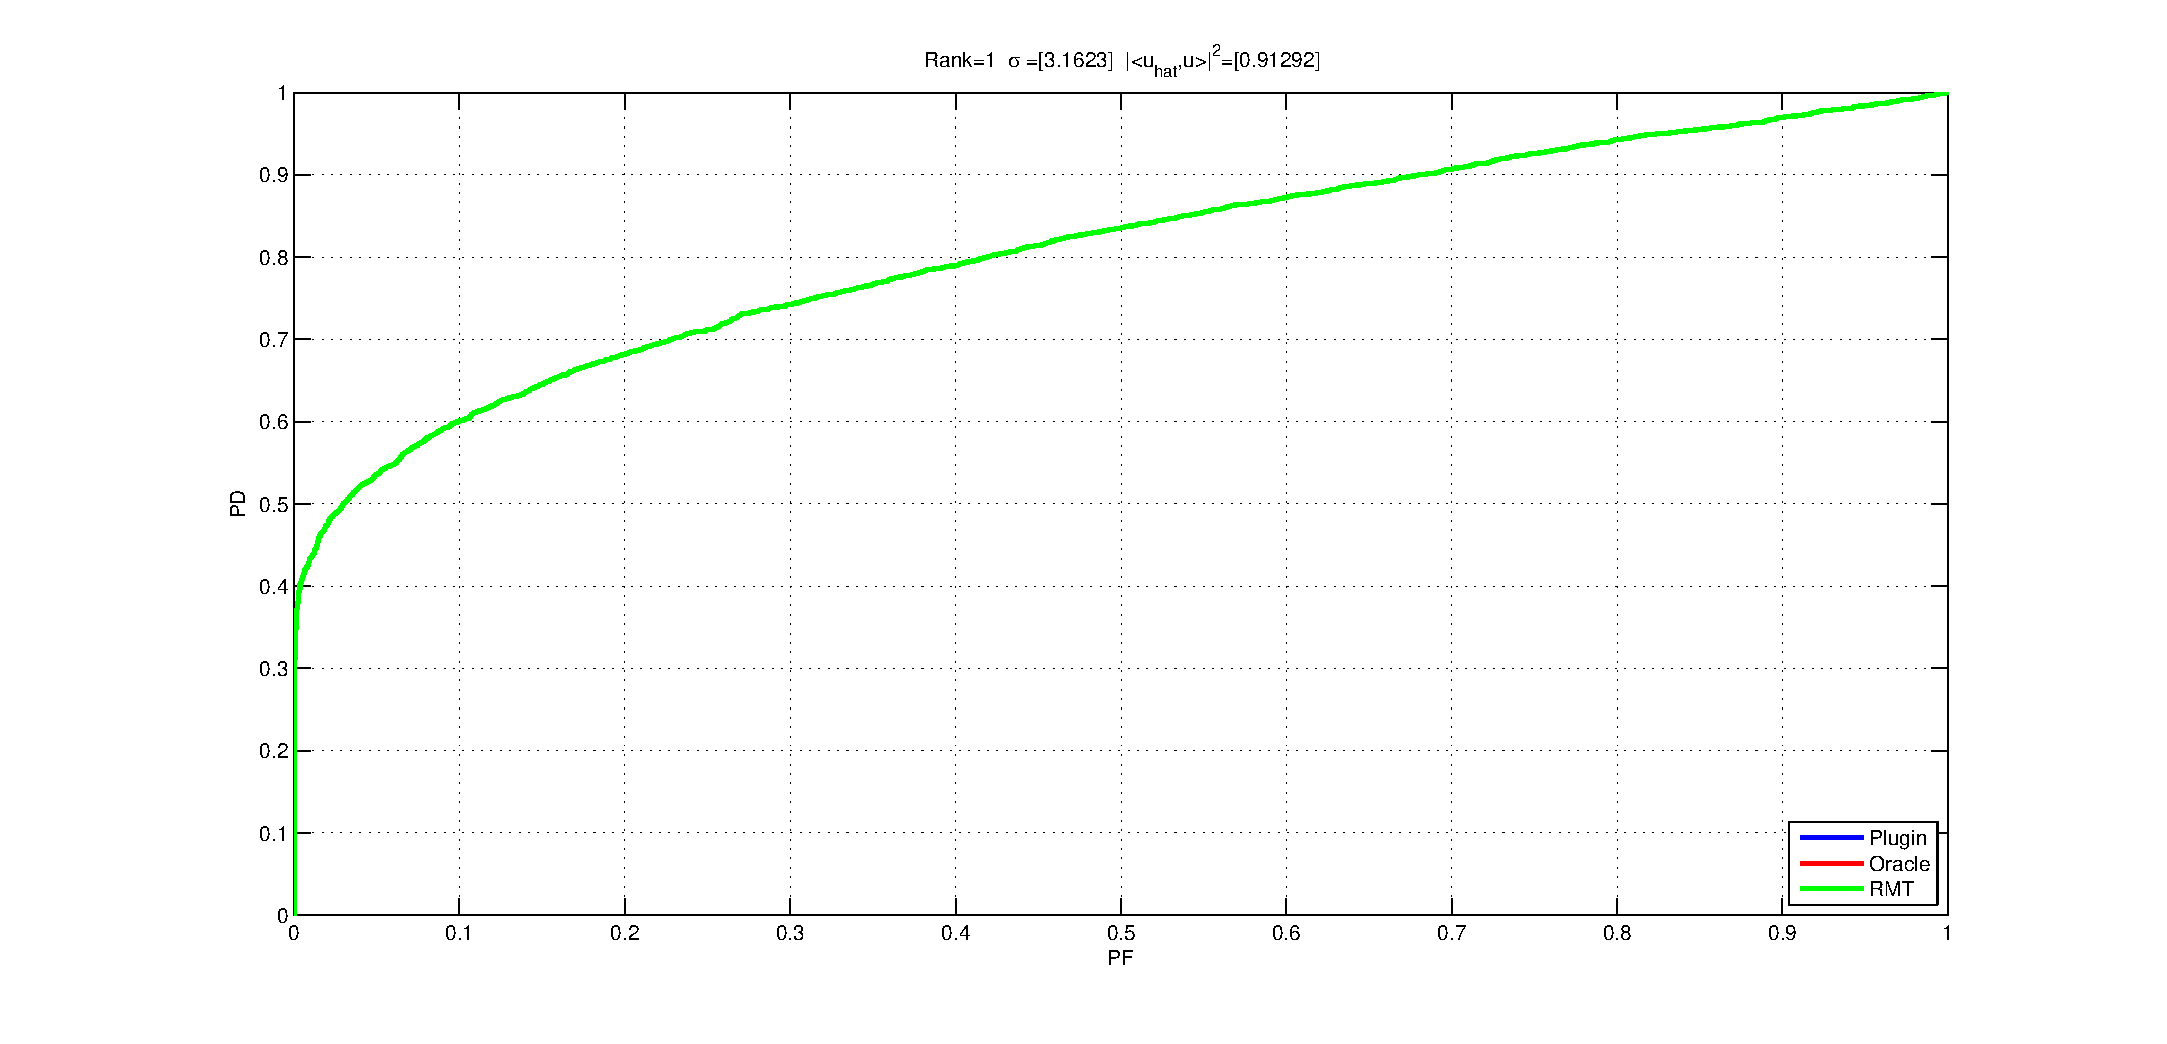
\includegraphics[width=5in]{rank_1}
\caption{Rank 1}
\end{figure}

\begin{figure}[h!]
\centering
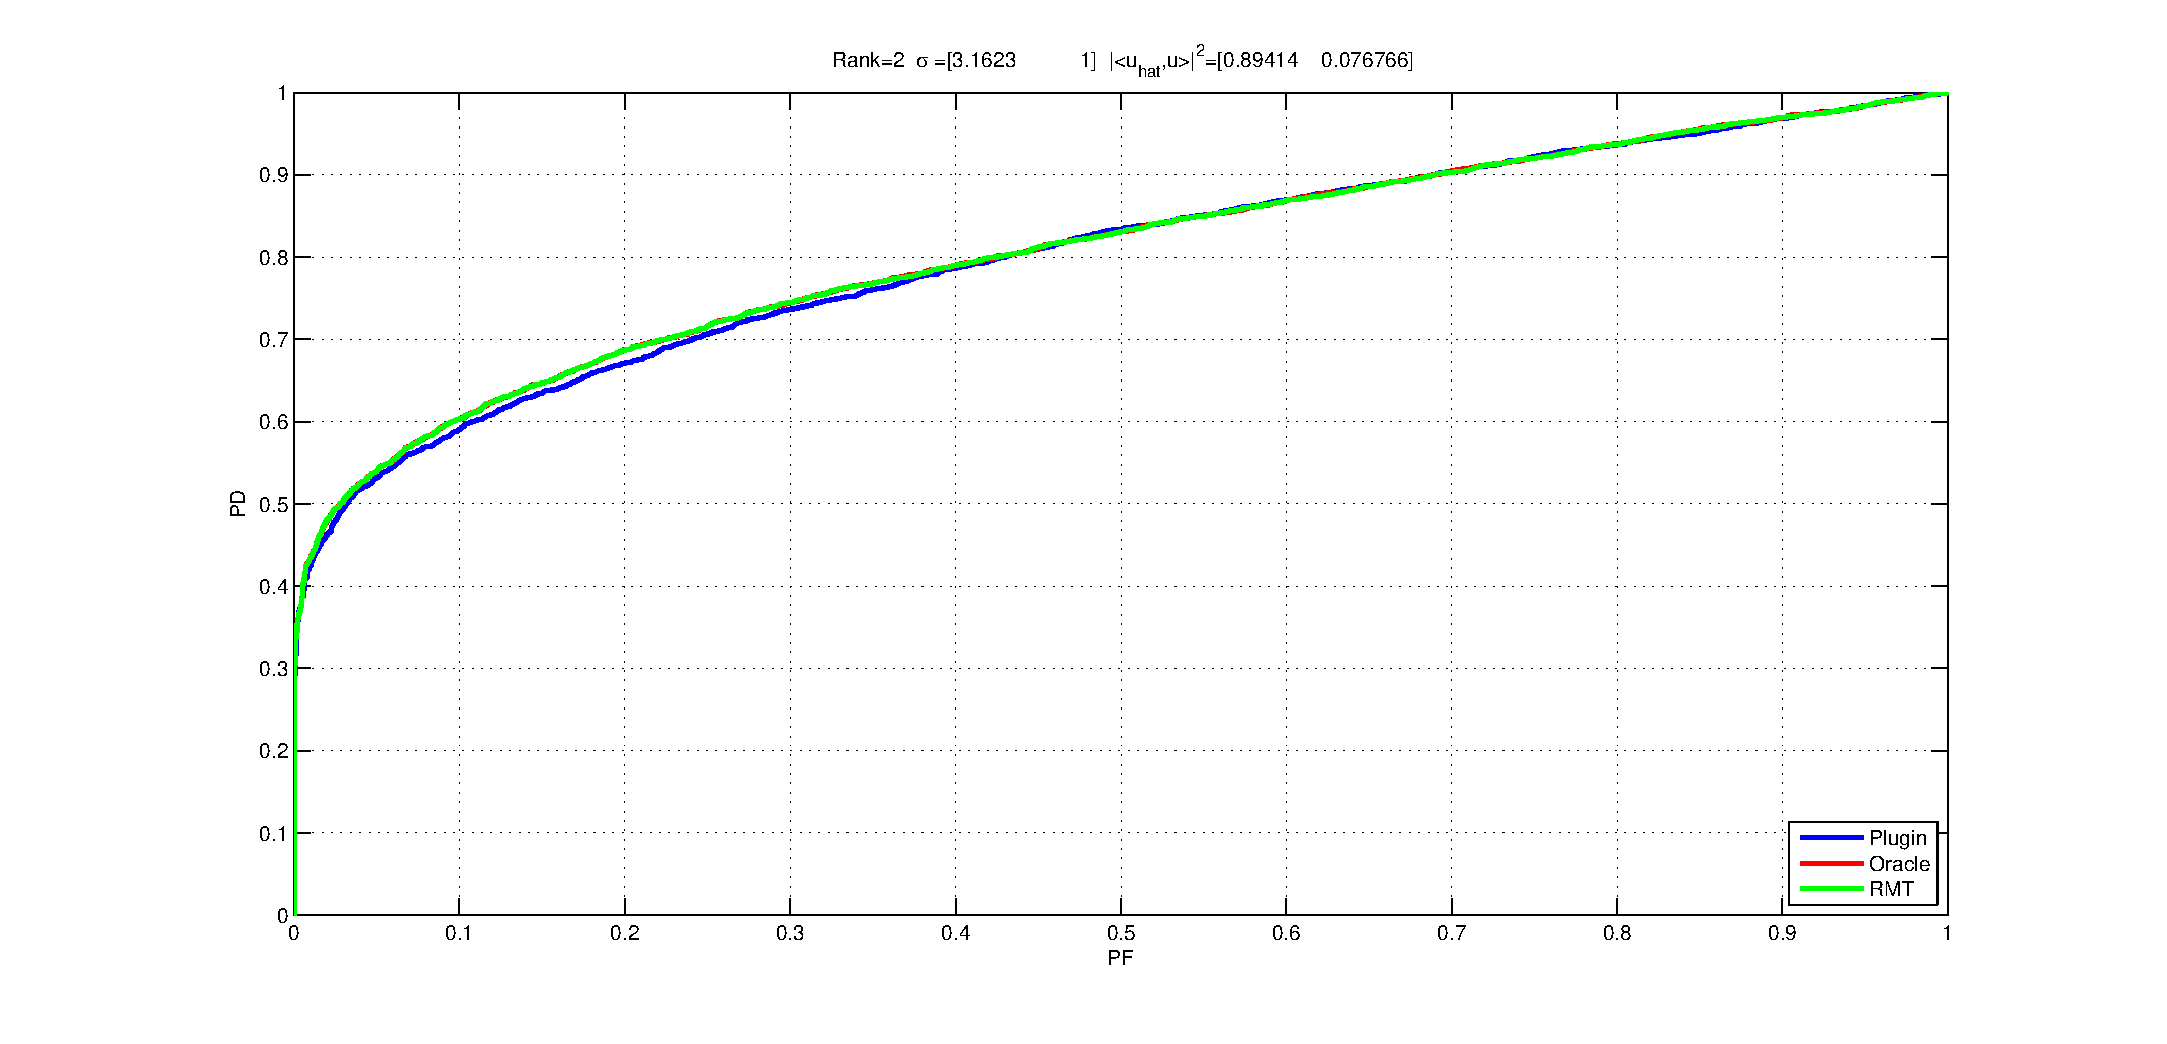
\includegraphics[width=5in]{rank_2}
\caption{Rank 2}
\end{figure}

\begin{figure}[h!]
\centering
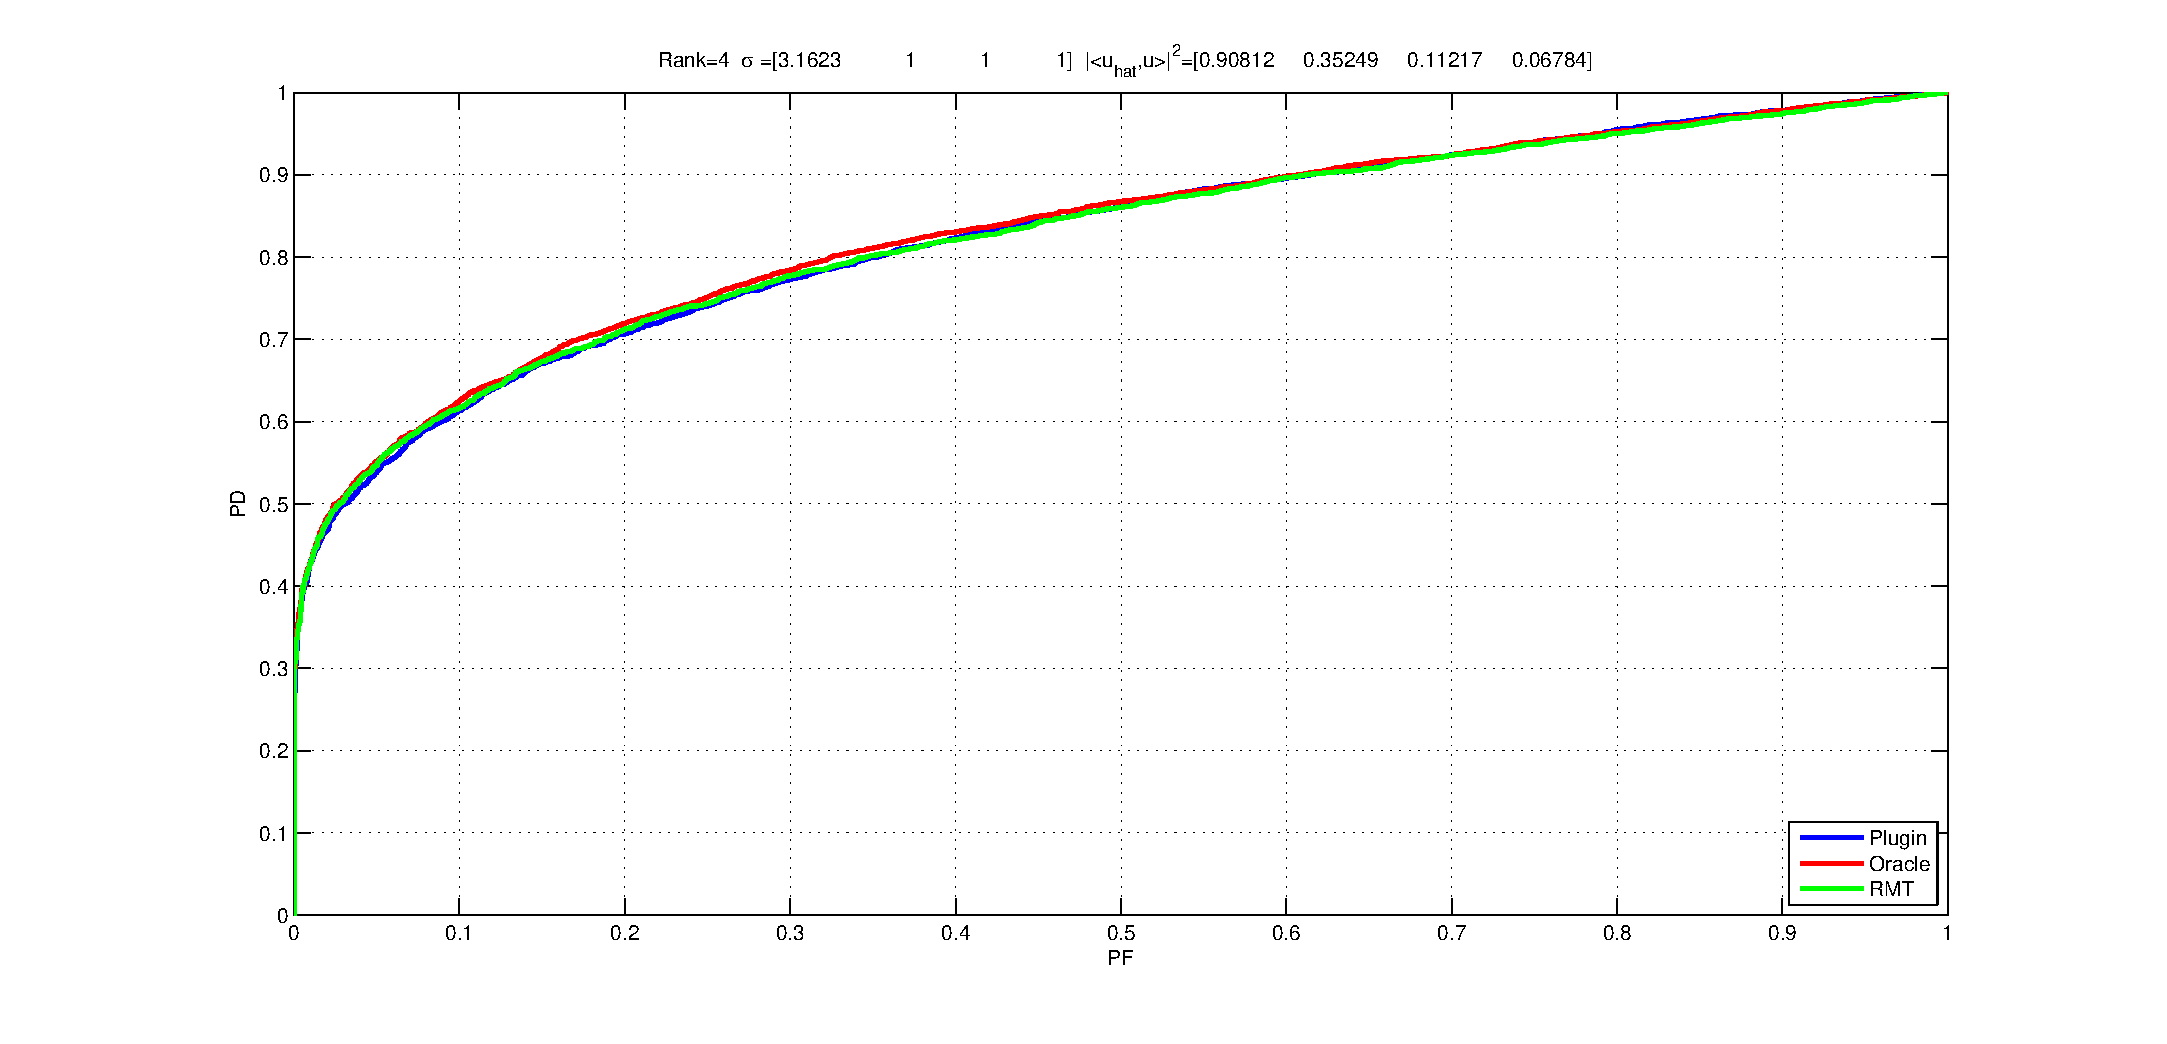
\includegraphics[width=5in]{rank_4}
\caption{Rank 4}
\end{figure}

\begin{figure}[h!]
\centering
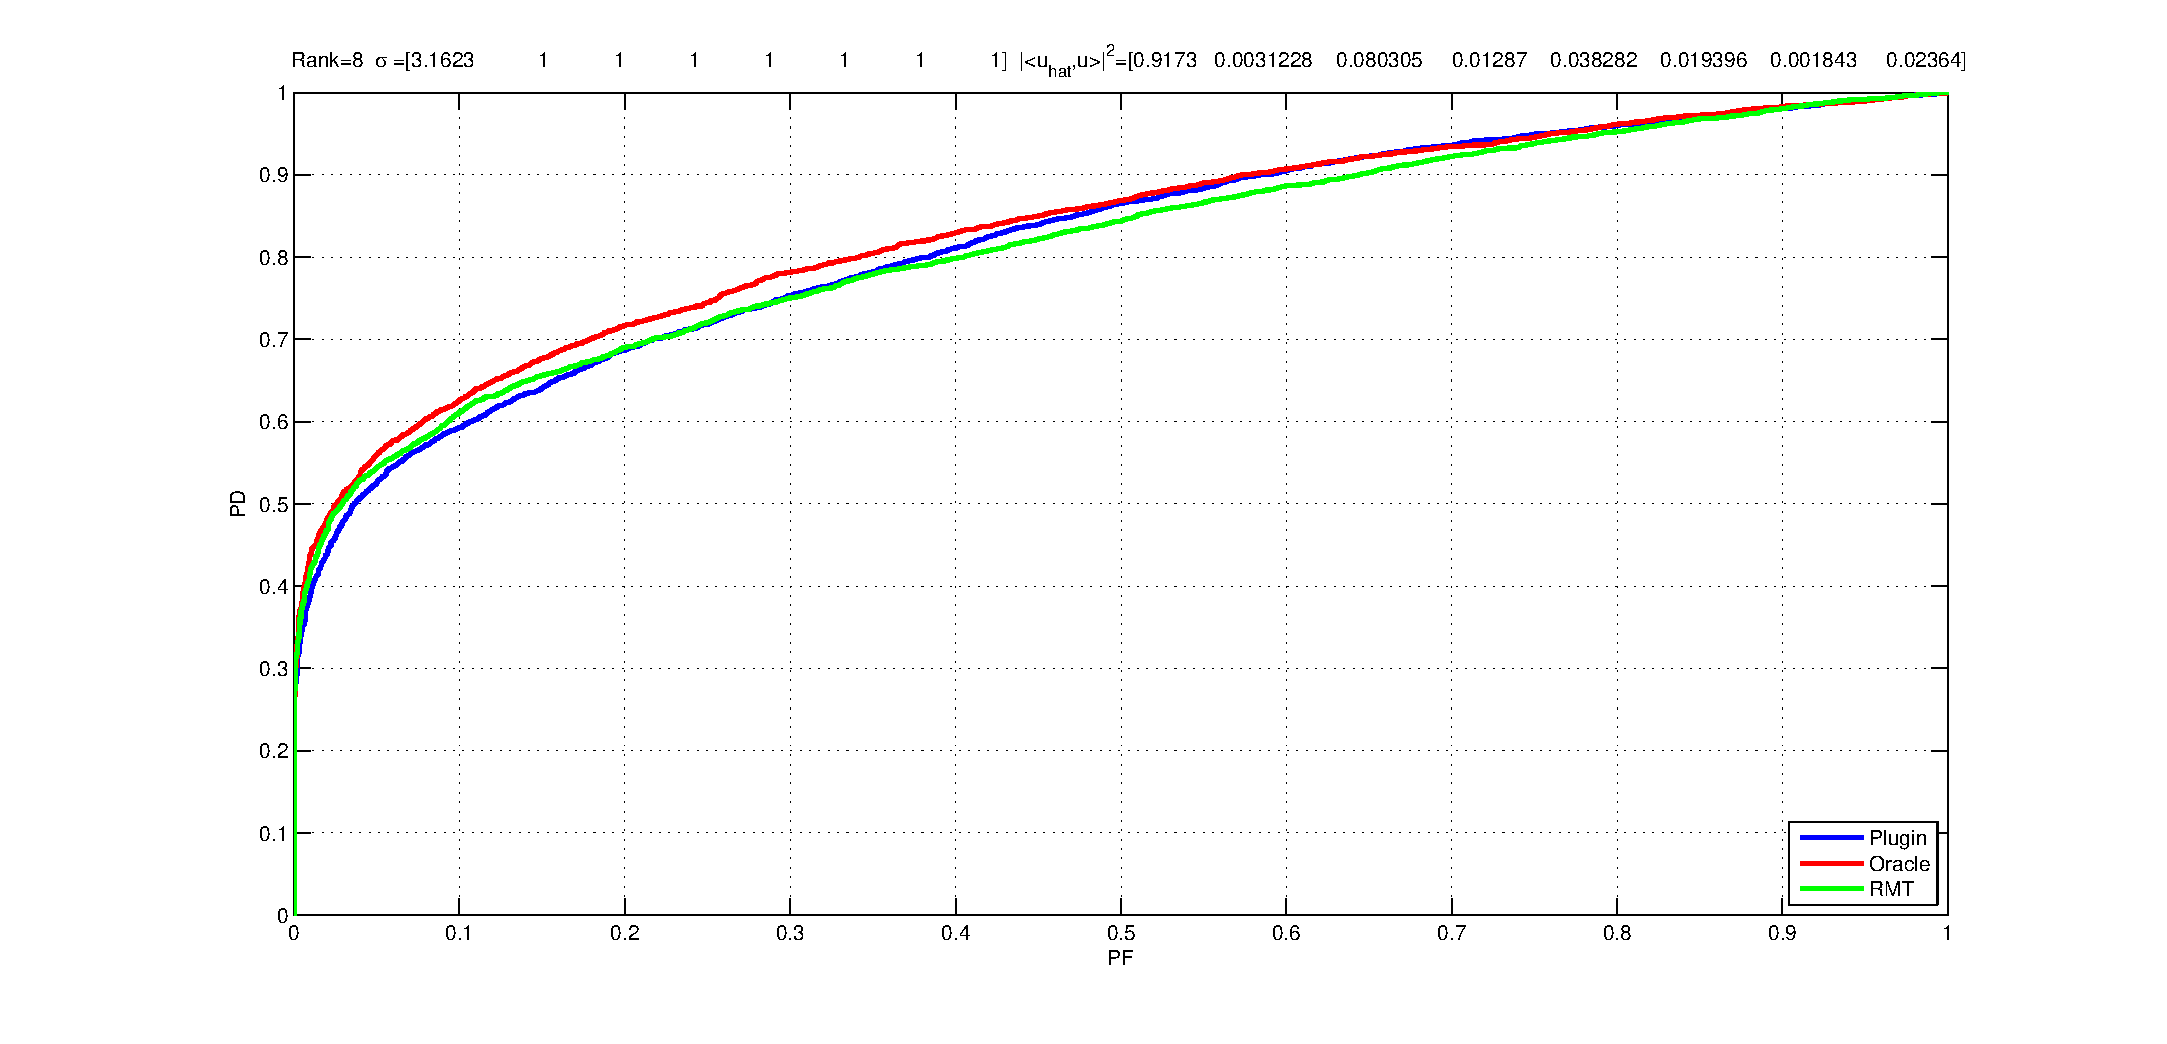
\includegraphics[width=5in]{rank_8}
\caption{Rank 8}
\end{figure}

\begin{figure}[h!]
\centering
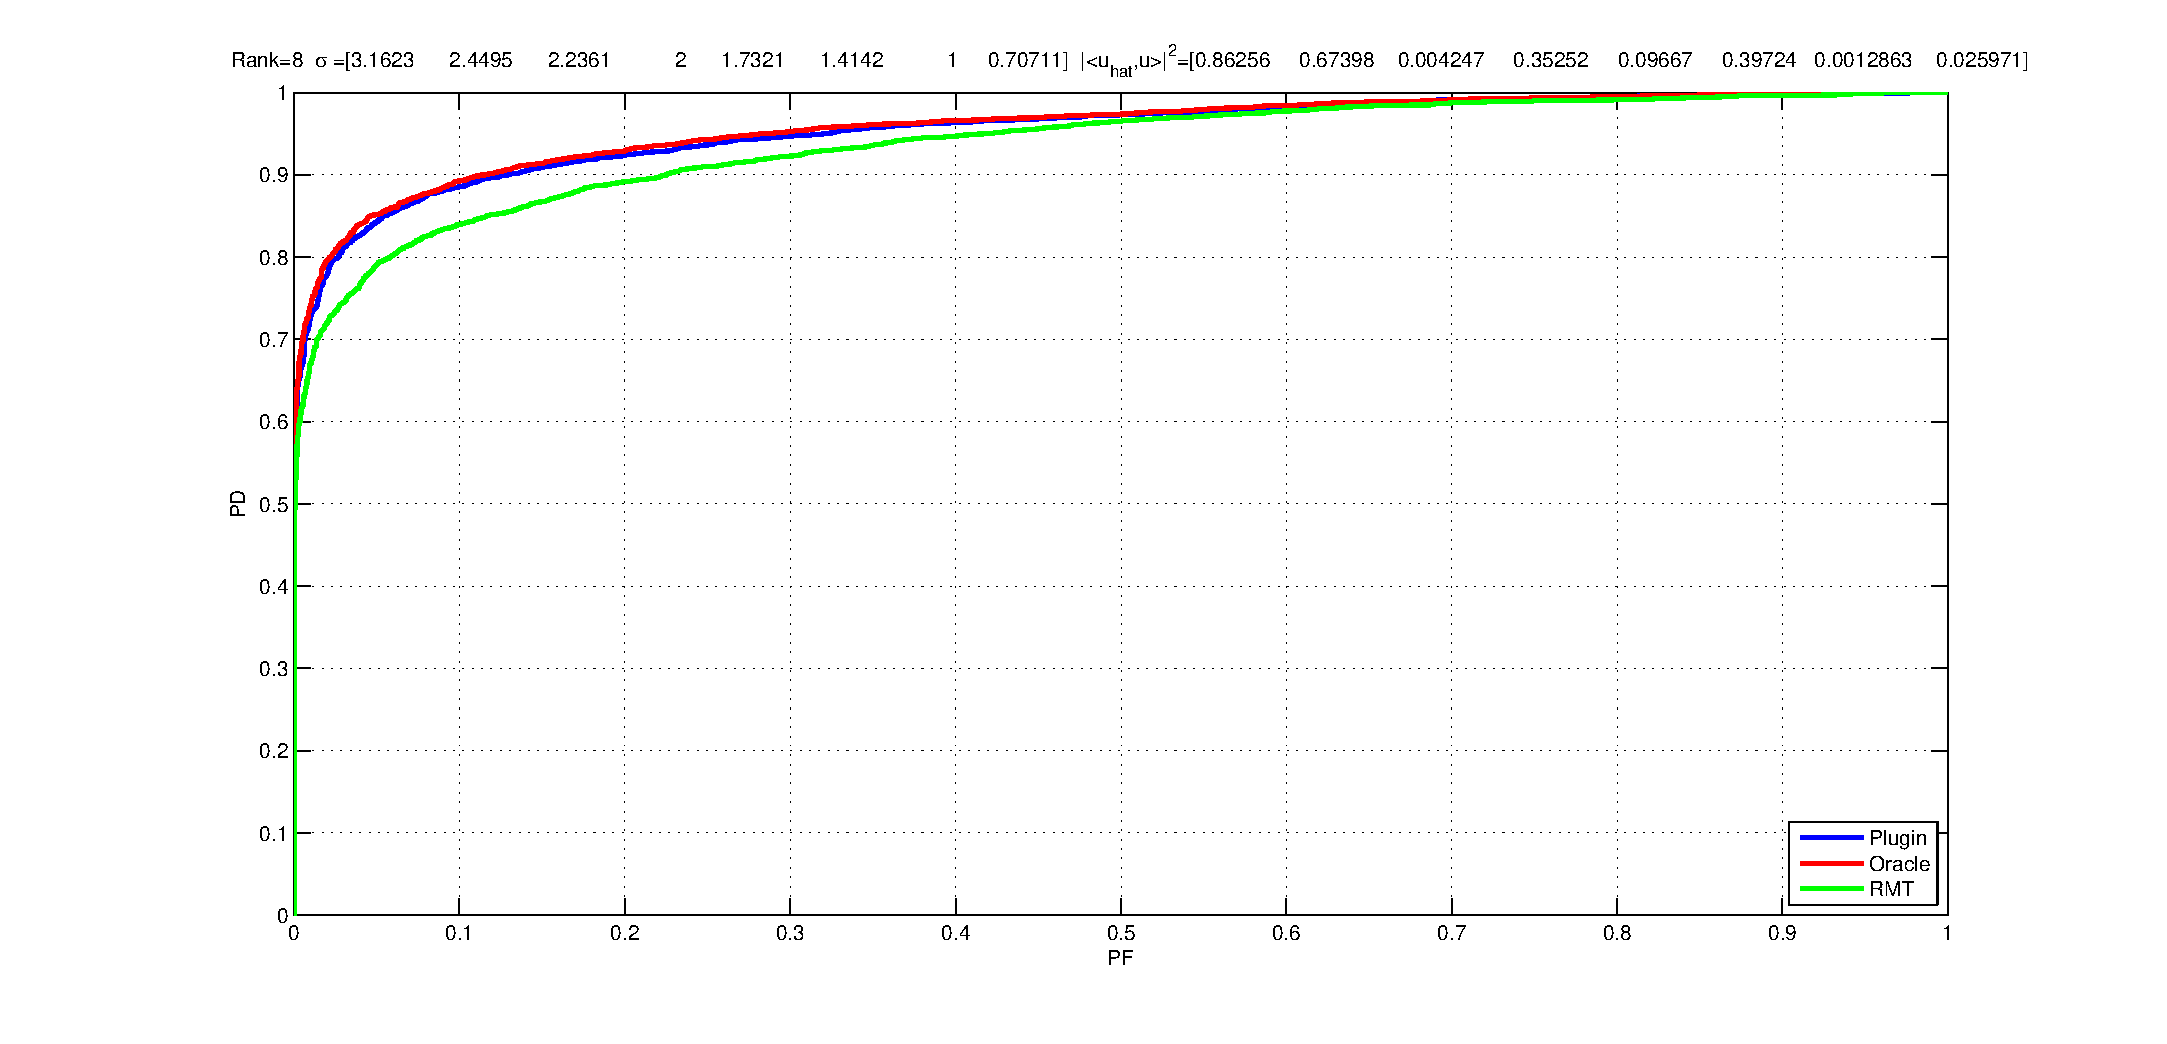
\includegraphics[width=5in]{rank_diff}
\caption{Rank 8 : decreasing $\sigma$}
\end{figure}

\end{document} 